\section{The adjudication: unattributed perturbation}
\label{sec:adjudication}

Section~\ref{sec:invivo} delivered the artifact; this section delivers
its verdict. The in-vivo-adapted file changes greedy continuations on
2 of 5 frozen prompts (both on the pre-registered low-margin subset),
and the question this section answers was fixed before any of it was
observed: \emph{are those changes attributable to the adaptation's
content, or would equal-dose random perturbation do the same?} The
answer, by a pre-registered decision rule, is the second. The term of
record for the adaptation's downstream effects is
\unattrib{}. This section shows the ladder that produced that ruling
--- and the false positive it caught, which was ours.

\subsection{The decision rule (committed before the evidence)}
\label{sec:rule}

The sequence of commitments is itself part of the method, and the
dates bind: the five judge prompts were frozen first; then a margin
census over every prompt$\times$step of the baseline dumps defined the
knife-edge set (top1$-$top2 margin $< \theta = 0.05$, keyed on
\emph{baseline} margins --- model properties before perturbation; the
patched side is an outcome, never a key); only then were the null
families generated and judged. Sibling prompts (weekday-triple
rotations, a month chain, length-matched off-circuit negatives, a
digit run) were rule-fixed before running, evidence-only.

The pre-registered conjunct: content-attribution survives \emph{only
if} all four arms hold ---
\begin{enumerate}
\item[(a)] the continuous statistic, $|\Delta\mathrm{margin}|$ at every
  knife-edge, for the in-vivo file exceeds the maximum over
  \emph{all} nulls;
\item[(b)] the null flip-rate on the knife-edge set is $\le 1/10$
  (escalation to $n{=}20$ at $0$--$1/10$, since the rule-of-three
  confidence interval at $n{=}10$ is too wide to carry the claim
  alone);
\item[(c)] the in-vivo dose curve exits the null band
  (mean\,$\pm$\,2SD) at every checkpoint;
\item[(d)] effects concentrate on the weekday set vs.\ off-circuit
  negatives.
\end{enumerate}
Any arm failing demotes the capability language --- recorded, not
debated.

\subsection{The null ladder}
\label{sec:ladder}

\paragraph{Primary family: dose-matched $\times$10.}
Each of ten draws changes \emph{exactly} 87{,}119 cells --- the H2
terminal dose --- with positions and values sampled from the H2
terminal diff (decoded from the patched artifact itself, never
re-run), region-matched, i.i.d.

\paragraph{The rung that cannot exist.}
The original design included a position-shuffle rung: keep H2's
changed-cell set, permute the assigned new-values (isolating content
from placement). Building it found a structural impossibility.

\begin{theorem}[Composition-specific null-feasibility]
\label{thm:shuffle}
H2's terminal diff has value multiset $\{0^{\,57{,}170},
+1^{\,29{,}949}\}$ --- it contains no $-1$s. Under the no-same-source
constraint (a permuted value must differ from its source), the
feasible assignment polytope is a single point: the 0-sourced demand
($29{,}949$) equals the entire $+1$ pool, forcing
$x[0\!\to\!+1] = 29{,}949$ and exhausting it; $-1$-sourced cells can
then only take 0s ($26{,}027$ forced); $+1$-sourced cells take the
remaining 0s ($31{,}143$ forced). H2's own mapping is the unique legal
assignment.
\end{theorem}

Empirical confirmation: a pairwise-exchange search returns zero legal
swaps; a greedy shuffle implementation produced a file
byte-identical to H2 (caught by sha before judging); a randomizing
implementation grinds forever on dead-end restarts. The consequence is
banked as a finding about the regime, not a workaround: \emph{at this
composition, content and placement are formally entangled} --- no
value-permutation null exists, and any future claim to separate what
was changed from where must first exit this composition. The rung was
redefined, pre-registered before any null table was read, as
\emph{value-flip $\times$3}: the real changed positions at exact dose,
each new value reflected where legal ($-1\!\to\!0$ becomes
$-1\!\to\!+1$, $+1\!\to\!0$ becomes $+1\!\to\!-1$;
$0\!\to\!+1$ has no legal reflection and stays) --- testing ``the
specific values matter,'' while changing the value multiset by design.

\paragraph{Stress arm (report-only).}
The project's first null family was census-matched to
\emph{transition} totals (1{,}112{,}771 flips $\approx$ 178k cells ---
flips are not cells; the terminal patch is 87{,}119). Discovered by
pre-mortem, it is relabeled a $\approx$2$\times$-dose stress arm:
context in the figures, never adjudication.

\subsection{The seals}
\label{sec:seals}

Three rules were sealed before the primary family's tables were read,
eliminating every remaining discretionary surface:
\begin{itemize}
\item \textbf{Seal 1 (void protocol):} a void is mechanical evidence
  only (non-zero exit or empty dump); re-run once; void twice
  $\to$ excluded with the denominator adjusted. The primary family
  recorded zero voids. (The stress arm's r10--p3 was void under this
  protocol --- warmup death --- correcting its banked table to 8/9
  valid.)
\item \textbf{Seal 2 (p4 bands):} $0$--$1/10$ dose-matched p4 flips
  $=$ thresholded; $\ge 5/10$ $=$ content-evidence; $2$--$4/10$ $=$
  MIXED --- reported, no p4 claim either way.
\item \textbf{Seal 3 (language pre-adjustment):} capability wording
  pre-weakened in the paper skeleton for \emph{both} outcome branches,
  so the ruling could not be felt in the prose.
\end{itemize}

\subsection{The primary family's evidence}
\label{sec:primary}

\begin{figure}[t]
\centering
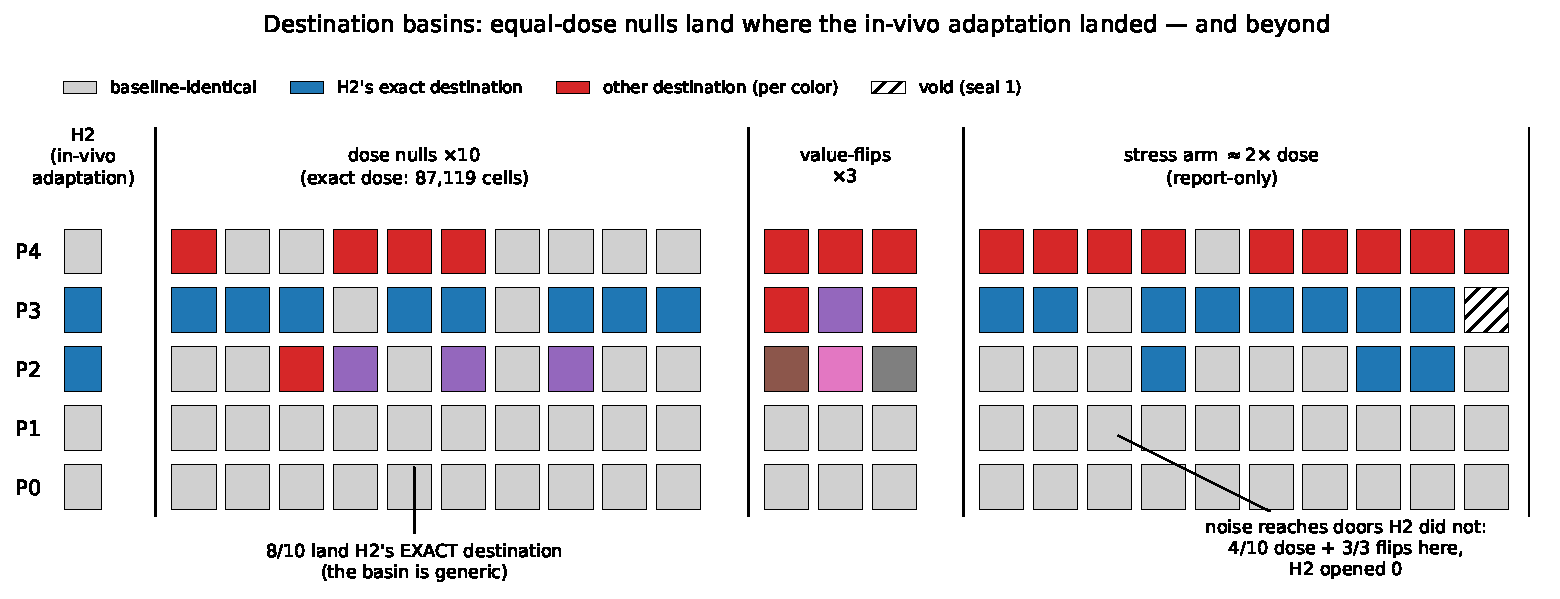
\includegraphics[width=\linewidth]{figs/basins.pdf}
\caption{Destination basins. Rows: judge prompts. Columns: the H2
(in-vivo) file, the ten dose-matched nulls, the three value-flip
nulls, and the report-only stress arm. Grey $=$ baseline-identical;
blue $=$ byte-identical to H2's continuation; other colors $=$ other
destinations; hatched $=$ void (seal 1). Eight of ten dose nulls land
H2's \emph{exact} p3 destination --- the basin is generic. Noise also
reaches doors H2 did not open (p4).}
\label{fig:basins}
\end{figure}

Figure~\ref{fig:basins} shows every draw's fate; the numbers here are
the README-recorded table the figure asserts against.

\paragraph{Flip counts.}
p0/p1: quiet everywhere (0/10, 0/3). p3: 8/10 dose nulls flip ---
\emph{and all eight land H2's exact destination} (``\,'Thursday' plus
ten newlines). p2: 4/10 (d3, d4, d6, d8). p4: 4/10 (d1, d4, d5, d6)
--- a MIXED band under seal 2: reported, no claim. Value-flips: p2
3/3, p3 3/3, p4 3/3.

\paragraph{Destinations --- p2's full denominator.}
The four dose-null p2 flips do \emph{not} form a degradation blob;
each destination is legible:
\begin{itemize}
\item \textbf{d3}: ``\ldots eleven twelve fifteen seventeen twenty
  one'' --- a \emph{different coherent odd chain}, not noise-salad;
\item \textbf{d4, d6, d8}: ``\ldots nine ten\,$\backslash$n\,What is
  the sum of'' --- the prompt's own trained continuation (the
  dead-wire-era basin), one line each; transcripts in
  Appendix~\ref{app:transcripts}.
\end{itemize}

\paragraph{The continuous statistic.}
At p3's step-1 knife-edge, H2 crosses the edge (margin $+0.0091 \to
-0.0707$) with $|\Delta\mathrm{margin}| = 0.0798$. The maximum over
all dose nulls at the same edge is $0.2254$ (null d6). Arm (a):
\textbf{FAIL} --- $0.0798 < 0.2254$. Arm (b): \textbf{FAIL} decisively
--- 8/10 null flips against a $\le 1/10$ bar; escalation is moot.
Arm (c): moot. Arm (d): MIXED per seal 2. The conjunct fails.

\subsection{The ruling}
\label{sec:ruling}

Branch B, by rule, zero discretionary calls: the in-vivo
adaptation's downstream effects fail every pre-registered criterion
for exceeding equal-dose random perturbation. \unattrib{} is the term
of record --- and two neighboring terms are explicitly refused:
\emph{degradation} is killed by d3's coherent chain (random
perturbation produced a \emph{different orderly continuation}, so
``degrades the model'' is not what random-walk-into-basins does), and
\emph{statistically indistinguishable} is refused because it claims an
unpowered equivalence this design never tested: the claim failed
pre-registered criteria, which is a refutation, not a tie.

Two footprint facts frame the ruling. H2's per-prompt footprint
$\{p2, p3\}$ sits \emph{inside} null experience --- noise reached
$\{p2, p3, p4\}$ (quantified in Sec.~\ref{sec:discussion}). And the
value-flips opened p4 3/3 where H2 opened 0 --- hypothesis-generating
only (the family changes the value multiset by design), but a pointer
to where content, if it exists, would have to show.

\subsection{The false positive we almost published}
\label{sec:averted}

The strongest evidence for the ladder is what it caught: us. The H1
run's judge result --- 11/12 argmax flips on the weekday prompt, a
complete continuation divergence after the shared first token --- was
recorded in the project's ledger, pre-adjudication, as:

\begin{quote}\small
``(i) STEERING demonstrated --- Tier-3's named stretch, achieved %%ALLOW%%
without widening'' %%ALLOW%% (verbatim quotation of the pre-adjudication reading; the term is retired)
\hfill --- project ledger, ISC-82, 2026-08-19
\end{quote}

Under the flip-count reading, that entry was a capability claim: the
in-vivo adaptation had moved the weekday prompt's dynamics decisively,
and four prior synthetic-era runs had shown 0/60 flips at this
footprint. The ladder then showed what the flips were made of: at
equal dose, random perturbation lands the same destination 8 times out
of 10. Flip-counts alone would have published a false positive; the
authors' first reading \emph{was} that false positive, and only the
pre-registered rule --- committed before the authors could see the
null tables --- reversed it. We report this openly because it is the
sharpest available demonstration of why the ladder's rungs (null
feasibility, destination basins, continuous statistics) are not
ceremony: they are what stands between a compelling count and a true
one.
